\documentclass{beamer}
\usetheme{default}
\setbeamercovered{transparent}
\setbeamertemplate{navigation symbols}{}
\setbeamertemplate{footline}{
  \flushright{\hfill \insertframenumber{}/\inserttotalframenumber}
}

\title{Introduction to \texttt{Bash}\\Setup \texttt{mk} modules and \texttt{git} repo}
\author{Pasquale Claudio Africa}
\institute{MOX\\ Dipartimento di Matematica\\
Politecnico di Milano}
\date{24/02/2022}

\usepackage{listings}

% Settings for listing class.
\lstset{  
  language=bash,                       % The default language
  basicstyle=\small\ttfamily,          % The basic style
  backgroundcolor=\color{white},       % Set listing background
  keywordstyle=\color{blue!50!black}\bfseries,  % Set keyword style
  commentstyle=\color{green!50!black}\itshape, % Set comment style
  stringstyle=\color{red!50!black},             % Set string constant style
  extendedchars=true                       % Allow extended characters
  breaklines=true,
  basewidth={0.5em,0.4em},
  fontadjust=true,
  linewidth=\textwidth,
  breakatwhitespace=true,
  showstringspaces=false,
  lineskip=0ex, %  frame=single
}

\setbeamertemplate{section in toc}[circle]
\AtBeginSection[]{%
    \begin{frame}{Outline}
        \tableofcontents[currentsection] 
    \end{frame}
}

\begin{document}

\begin{frame}
    \titlepage
\end{frame}

\begin{frame}{Practical info}
    Lab sessions:\\
    Friday 13:15 -- 16:15, room 7.0.1
    \vfill
    Webex room: \\
    \url{https://politecnicomilano.webex.com/meet/pasqualeclaudio.africa}
    \vfill
    Email: \href{mailto:pasqualeclaudio.africa@polimi.it}{pasqualeclaudio.africa@polimi.it}.
    \vfill
    Use the \href{https://webeep.polimi.it/mod/forum/view.php?id=2521}{WeBeep Forum} for general questions.
\end{frame}

\begin{frame}{Outline}
    \tableofcontents
\end{frame}

\section{\texttt{Bash}}
\begin{frame}{What is a shell?}
    \begin{center}
        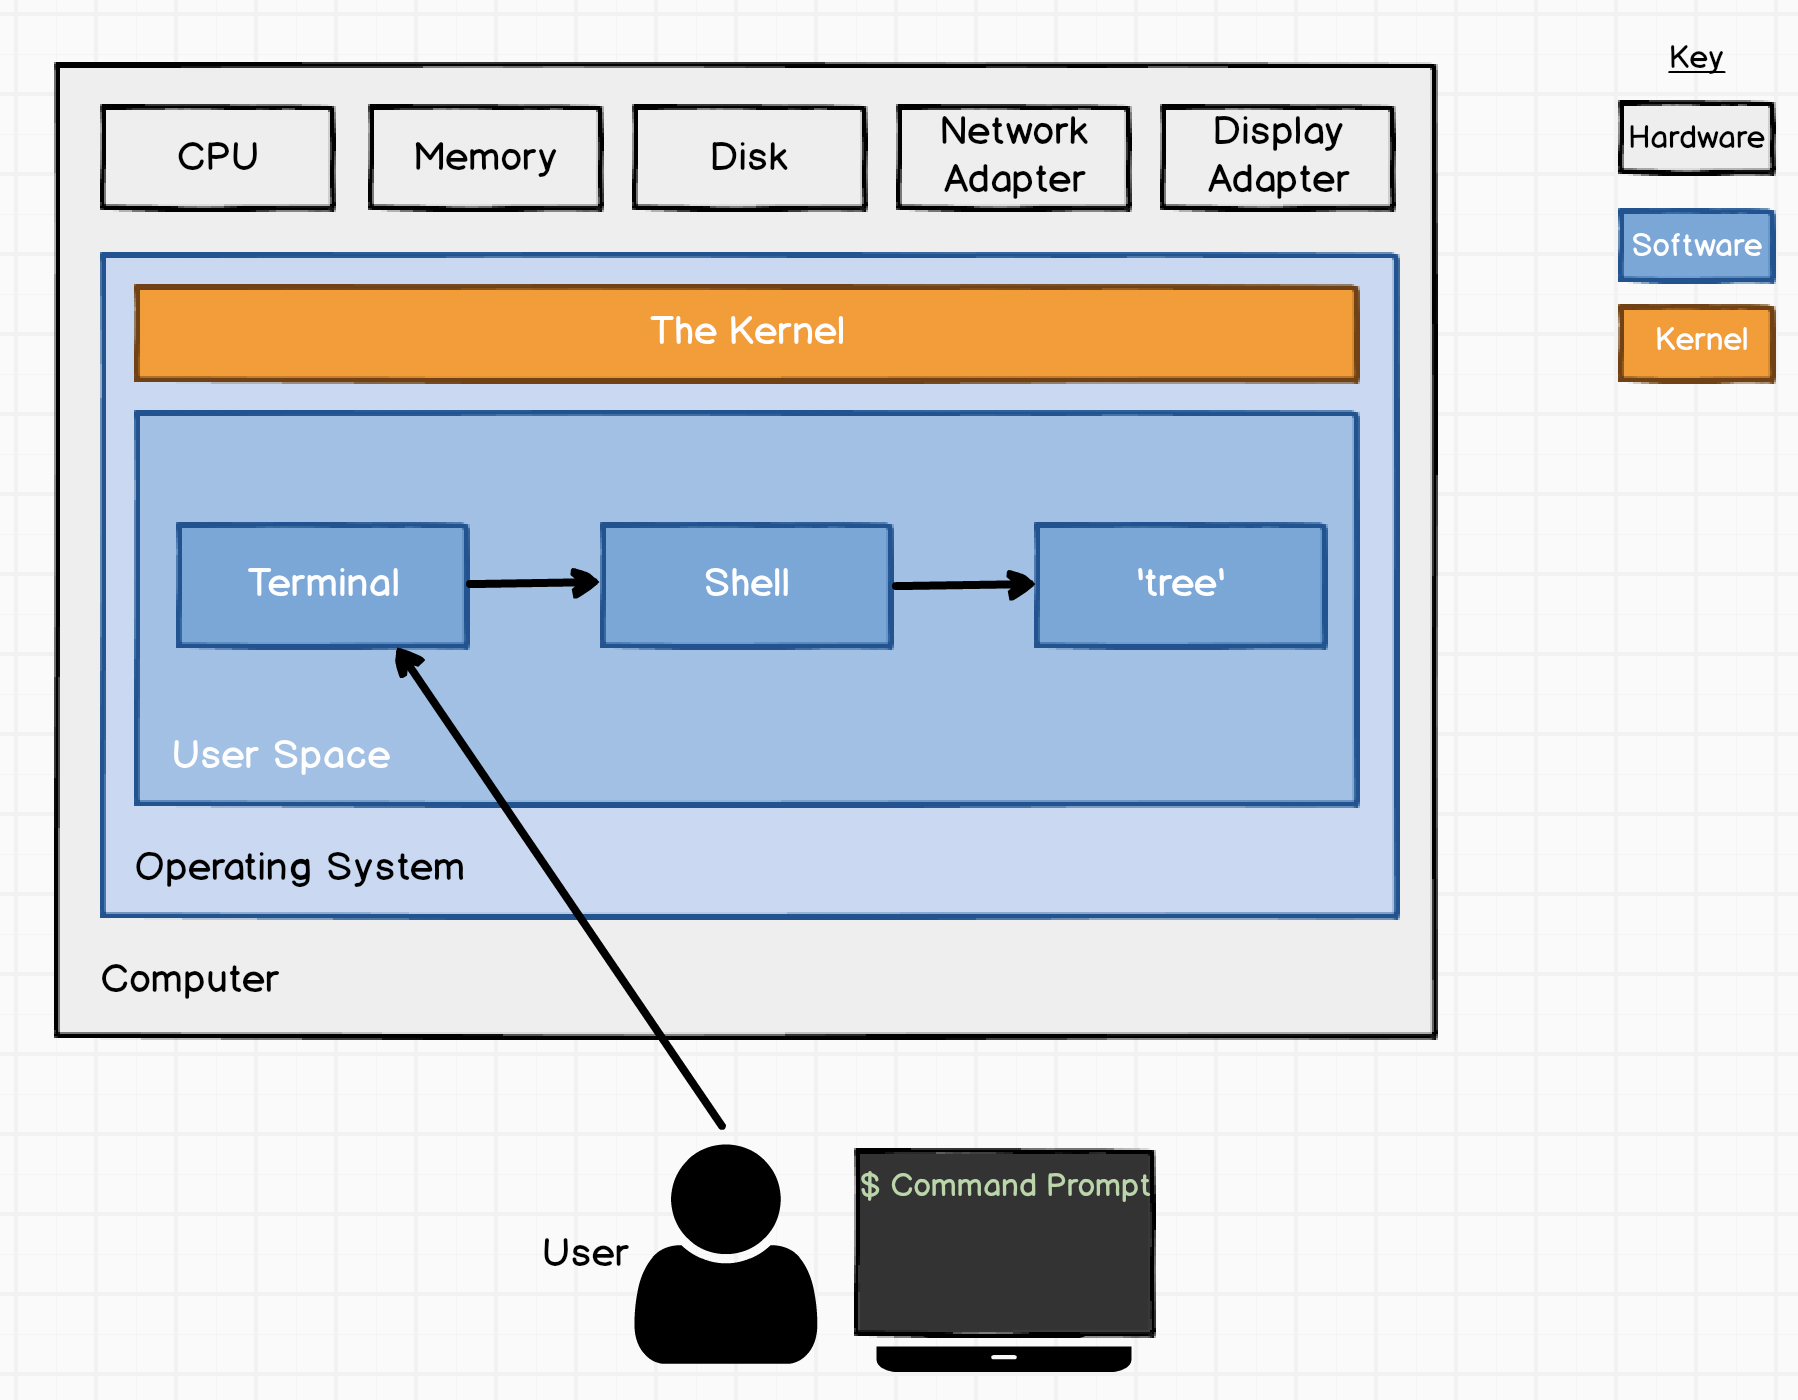
\includegraphics[width=\textwidth]{shell.png}
    \end{center}
\end{frame}

\begin{frame}{What is a shell?}
    From \url{http://www.linfo.org/shell.html}:
    \textit{``A shell is a program that provides the traditional, text-only user interface for Linux and other Unix-like operating systems. Its primary function is to read commands that are typed into a console (i.e., an all-text display mode) or terminal window (an all-text window) in a GUI (graphical user interface) and then execute (i.e., run) them.\\
    The term shell derives its name from the fact that it is an outer layer of an operating system. A shell is an interface between the user and the internal parts of the operating system (at the very core of which is the kernel).''}
\end{frame}

\begin{frame}{What is \texttt{Bash}?}

  \texttt{Bash} stands for: \texttt{Bourne Again Shell}, a homage to its creator Stephen Bourne.
  \vfill
  It is the default shell for most Unix systems and Linux distributions. \\
  It is also available for \href{https://docs.microsoft.com/it-it/windows/wsl/about}{Windows 10} since 2016. \\
  macOS has replaced it with \href{https://support.apple.com/en-us/HT208050}{\texttt{zsh}}, which is mostly compatible with \texttt{Bash}, since v10.15 Catalina.
  \vfill
  It is both a command interpreter and a scripting language.
  \vfill
  Alternatives: \texttt{csh}, \texttt{zsh}, \texttt{ksh}, \dots\\
  The shell might be changed by simply typing its name and even the default shell might be changed for all sessions.
\end{frame}

\begin{frame}{Types of shell}
    \small
    \begin{itemize}
        \item A \textbf{login} shell logs you into the system as a specific user (it requires username and password). When you hit \texttt{Ctrl+Alt+F1} to login into a virtual terminal you get after successful login: a login shell (that is interactive).
        \item A \textbf{non-login} shell is executed without logging in (it requires a current logged in user). When you open a graphic terminal it is a non-login (interactive) shell. 
        \item In an \textbf{interactive} shell (login or non-login) you can interactively type or interrupt commands. For example a graaphic terminal (non-login) or a virtual terminal (login). In an interactive shell the prompt variable must be set (\texttt{\$PS1}).
        \item A \textbf{non-interactive} (sub)shell is usually run from an automated process. Input and output are not exposed (unless explicitly handled by the calling process). This is normally a non-login shell, because the calling user has logged in already. A shell running a script is always a non-interactive shell (but the script can emulate an interactive shell by prompting the user to input values).
    \end{itemize}
\end{frame}

\begin{frame}{\texttt{Bash} as a command interpreter}
When launching a terminal a Unix system first launches the shell interpreter specified in the \texttt{SHELL} \textbf{environment variable}. If \texttt{SHELL} is unset it uses the system default.
\vfill
After having sourced the initialization files, the interpreter shows the \textbf{prompt} (defined by the environment variable \texttt{\$PS1}).
\vfill
Initialization files are hidden files stored in the user's home directory, executed as soon as an \textbf{interactive} shell is run:
\begin{itemize}
    \item \textbf{login}: the first readable file among \texttt{\~{}/.bash\_profile}, \texttt{\~{}/.bash\_login}, \texttt{\~{}/.profile}, in that order;
    \item \textbf{non-login}: \texttt{\~{}/.bashrc}
\end{itemize}
\end{frame}

\begin{frame}{Initialization files (in more detail)}
    \small
    \begin{itemize}
        \item \textbf{login}:
        \begin{itemize}
            \item \texttt{/etc/profile}, \texttt{/etc/profile.d/*}, \texttt{\~{}/.profile} for Bourne-compatible shells
            \item \texttt{\~{}/.bash\_profile} (or \texttt{\~{}/.bash\_login}) for \texttt{Bash}
            \item \texttt{/etc/zprofile}, \texttt{\~{}/.zprofile} for \texttt{zsh}
            \item \texttt{/etc/csh.login}, \texttt{\~{}/.login} for \texttt{csh}
        \end{itemize}        

        \item \textbf{non-login}: \texttt{/etc/bash.bashrc}, \texttt{\~{}/.bashrc} for \texttt{Bash}

        \item \textbf{interactive}:
        \begin{itemize}
            \item \texttt{/etc/profile}, \texttt{/etc/profile.d/*} and \texttt{\~{}/.profile}
            \item \texttt{/etc/bash.bashrc}, \texttt{\~{}/.bashrc} for \texttt{Bash}
        \end{itemize}

        \item \textbf{non-interactive}:
        \begin{itemize}
            \item \texttt{/etc/bash.bashrc} for \texttt{Bash} (but most of the times the script begins with: \texttt{[ -z "\$PS1" ] \&\& return}, \textit{i.e.} don't do anything if it's a non-interactive shell).
            \item depending on the shell, the file specified in the \texttt{\$ENV} (or \texttt{\$BASH\_ENV}) variable might be read.
        \end{itemize}
    \end{itemize}
\end{frame}

\begin{frame}{Sourcing a script and launching a subprocess}
When executing a command, like \texttt{ls} (\textit{list files}) a subprocess is created. A subprocess inherits all the environment variables from the parent process, executes the command and returns the control to the calling process.
\vfill
\underline{A subprocess cannot change the state of the calling process}.
\vfill
The command \texttt{source script\_file} executes the commands contained in \texttt{script\_file} as if they were typed directly on the terminal. It is only used on scripts that have to change some environmental variables or define aliases or function. \\
Typing \texttt{.\ script\_file} does the same.
\vfill
If the environment should not be altered, use \texttt{./script\_file}, instead.
\end{frame}

\begin{frame}{Filenames}
In order to live happily and without worries, \textbf{don't} use spaces in filenames!
\vfill
Space characters in file names should be forbidden by law! The space is used as separation character, having it in a file name makes things a lot more complicated in any script (not just \texttt{bash} scripts).
\vfill
Use underscores (snake case): \texttt{my\_wonderful\_file\_name}, or uppercase characters (camel case): \texttt{myWonderfulFileName}, or hyphens: \texttt{my-wonderful-file-name}, or a mixture:
\texttt{myWonderful\_file-name}, instead.
\vfill
But \textbf{not} \texttt{my wonderful file name}. It is not wonderful at all if it has to be parsed in a script.
\end{frame}

\begin{frame}{Builtin commands}
Some commands, like \texttt{cd} (change directory) are executed directly by the shell, without creating a subprocess.
\vfill
Indeed it would be impossible the have \texttt{cd} as a regular command! Why?
\vfill
\pause
\textbf{Answer}: a subprocess cannot change the state of the calling process, whereas \texttt{cd} needs to change the value of the environmental
variable \texttt{PWD} (that contains the name of the current working directory).
\end{frame}

\begin{frame}[fragile]{Main commands}
\begin{lstlisting}
cd dirname           # Change directory.
cd ~; cd ${HOME}; cd # Go to home directory.
cd -                 # Go back to previous directory.

mkdir dirname # Create directory.

ls           # List file and folders.
ls -l; ls -A # List file showing details or hidden files.

rm filename; rm -f filename # Remove file (forcingly).
rm -r dirname               # Recursively remove directory.

mv source dest # Rename/move file.

cat filename                 # Print content of file.
more filename; less filename # Print file page by page.
grep "string" filename       # Find string in a file.
\end{lstlisting}
\end{frame}

\begin{frame}[fragile]{Commands, builtins, aliases, functions, \dots}
In general a \textbf{command} can refer to:
\begin{itemize}
    \item a builtin command;
    \item an executable;
    \item an alias;
    \item a function.
\end{itemize}
\vfill
The shell looks for executables with a given name within directories specified in the environment variable \texttt{PATH}, whereas aliases and functions are usually sourced by the \texttt{.bashrc} file (or equivalent).
\vfill
To check what \texttt{command\_name} is:
\begin{lstlisting}
type command_name
\end{lstlisting}
\end{frame}

\begin{frame}[fragile]{Aliases}
\begin{lstlisting}
alias ls='ls -l'

unalias ls # Delete an alias.
\end{lstlisting}
\end{frame}

\begin{frame}[fragile]{Functions}
\begin{lstlisting}
function hello_world {
  echo "Hello, world!"
}

unset hello_world # Delete a function.
\end{lstlisting}
\vfill
The input arguments are referred to as \texttt{\$1}, \texttt{\$2}, \dots, \texttt{\$n}. \texttt{\$0} is reserved for the function name. \texttt{\$\#} holds the number of arguments. \texttt{\$*} and \texttt{\$@} hold all input arguments (\texttt{"\$*"} expands to \texttt{"\$1 \$2 \$n"}, whereas \texttt{"\$@"} to \texttt{"\$1" "\$2" "\$n"}).
\begin{lstlisting}
function print_something {
  echo "No. input arguments: $#"
  echo "First argument: $1"
  echo "All arguments: $*"
}
\end{lstlisting}
\end{frame}

\begin{frame}[fragile]{\texttt{if} clause}
\begin{columns}[t]
    \begin{column}{0.35\textwidth}
    \begin{lstlisting}
test EXPRESSION
[ EXPRESSION ]
[[ EXPRESSION ]]



if TEST_EXPRESSION
then
    STATEMENT
elif TEST_EXPRESSION2
    STATEMENT2
else
    STATEMENT3
fi
    \end{lstlisting}
    \end{column}
    \begin{column}{0.65\textwidth}
    \begin{lstlisting}[basicstyle=\scriptsize]
! EXPRESSION # EXPRESSION is false.

-n STRING # STRING is non-empty.
-z STRING # STRING is empty.
STRING1 == STRING2
STRING1 != STRING2

INTEGER1 -eq INTEGER2 # Equal to.
INTEGER1 -gt INTEGER2 # Greater than.
INTEGER1 -lt INTEGER2 # Less than.

INTEGER1 -ne INTEGER2 # Not equal to.
INTEGER1 -ge INTEGER2 # Greater than or equal to.
INTEGER1 -le INTEGER2 # Less than or equal to.

-d DIR  # Directory DIR exists.
-e FILE # FILE exists.
-s FILE # FILE exists and it is not empty.
-r FILE # FILE exists and it is readable.
-w FILE # FILE exists and it is writable.
-x FILE # FILE exists and it is executable.
    \end{lstlisting}
    \end{column}
\end{columns}
\end{frame}

\begin{frame}[fragile]{Redirection}
Redirect the standard output to file:
\begin{lstlisting}
command_name > output.log
\end{lstlisting}
\vfill
Redirect the standard error to file:
\begin{lstlisting}
command_name 2> error.log
\end{lstlisting}
\vfill
Redirect both the standard output and the standard error to file:
\begin{lstlisting}
command_name > output.txt 2>&1

# Or, equivalently:
command_name &> output.txt
\end{lstlisting}
\end{frame}

\begin{frame}[fragile]{Pipes}
One of the most powerful feature of \texttt{Bash} (and other shells) are pipes, which allow to transfer the output of a command as an input to another command:
\begin{lstlisting}
cat foo.txt | tr [a-z] [A-Z] > FOO.TXT
grep "old" settings.ini | sed -s "s/old/new/g"
\end{lstlisting}
The first command stores in \texttt{FOO.TXT} the content of the file \texttt{foo.txt} with lowercase letters converted to uppercase. The second command prints on the screen the lines of \texttt{settings.ini} with all occurrences of \texttt{old} replaced by \texttt{new}.
\end{frame}

\begin{frame}{More about pipes}
The \texttt{A \&\& B} pipe is activated only if the return status of \texttt{A} is 0.
\vfill
The \texttt{A || B} pipe is activated only if the return status of \texttt{A} is different from 0.
\vfill
\texttt{A; B} executes \texttt{A} and then \texttt{B}, regardless the return status of \texttt{A}.
\vfill
The return value of the last executed command is stored in \texttt{\$?}.
\end{frame}

\begin{frame}[fragile]{Regular and environment variables}
A variable may be defined with
\begin{lstlisting}
a="this is a variable"
unset a # Delete a variable.
\end{lstlisting}
\vfill
A variable is recalled by prepending the dollar sign and, optionally, enclosing within braces:
\begin{lstlisting}
echo $variable
echo ${variable_name} # Safer, as it prevents ambiguity.
\end{lstlisting}
\vfill
Environment variables are special variables that are available to subprocesses too. They are defined using the builtin command \texttt{export}:
\begin{lstlisting}
export a="this is an environment variable"
export PATH=/bin:/usr/bin:/usr/local/bin:${PATH}
\end{lstlisting}
\end{frame}

\begin{frame}[fragile]{\texttt{Bash} as a scripting language}
\begin{lstlisting}
#!/bin/bash

# This variable is global and can be used
# anywhere in this script.
VAR="global variable"

# We are hiding the system "bash" command!
function bash {
  # This variable is local to this function only.
  local VAR="local variable"
  echo $VAR
}

echo $VAR
bash

echo $VAR
\end{lstlisting}
\end{frame}

\begin{frame}[fragile]{Quotes}
Double quotes may be used to identify a string where the variables
are interpreted. Single quotes identify a string where variables are not interpreted.
\begin{lstlisting}
a=yes
echo "$a"
echo '$a'
\end{lstlisting}
The output of a command can be converted into a string and assigned to a variable for later reuse:\\
\texttt{list=\`{}ls -l\`{}}, or\\
\texttt{list=\$(ls -l)}
\end{frame}

\begin{frame}[fragile]{Processes}
Launch a command and send it in the background:
\begin{lstlisting}
./my_command &
\end{lstlisting}

\begin{itemize}
\item \texttt{Ctrl-Z} suspends the current subprocess and \texttt{bg} reactivates the suspended subprocess in the background.

\item \texttt{jobs} lists all subprocesses running in the background in the terminal.

\item \texttt{fg \%n} brings back to the foreground the n-th subprocess in the background.

\item \texttt{Ctrl-C} terminates the subprocess in the foreground (when not trapped).

\item \texttt{kill \%n} sends termination signal to the n-th subprocess.
\end{itemize}

All subprocesses in the background of the terminal are terminated when the terminal is closed (unless launched with \texttt{nohup}, but that is another story\dots)
\end{frame}

\begin{frame}[t,fragile]{Finding files: \texttt{find}}
\vspace{0.5cm}
\begin{overlayarea}{\textwidth}{0.15\textheight}
Two main commands are available for finding files: \texttt{find} and \texttt{locate}.
\end{overlayarea}
\vspace{0.5cm}
The first is a very powerful command that searches files in the specified directories that meet certain conditions, \textit{e.g.}
\begin{lstlisting}
find ~ -type f -mtime -3
\end{lstlisting}
finds all files (not directories) starting from my home directory (\texttt{\~{}}) that have been modified less than 3 hours ago.
\begin{lstlisting}
find . -type d -name "*lib*"
\end{lstlisting}
find all directories (not files) starting from the current one (\texttt{.}) whose name contain \texttt{lib}.
\end{frame}

\begin{frame}[t,fragile]{Finding files: \texttt{locate}}
\vspace{0.5cm}
\begin{overlayarea}{\textwidth}{0.15\textheight}
    Two main commands are available for finding files: \texttt{find} and \texttt{locate}.
\end{overlayarea}
\vspace{0.5cm}
The command \texttt{locate} is less powerful than \texttt{find} but much faster since it relies on a database that is updated on a daily base or manually using the command \texttt{updatedb} (administrator privileges required).
\vfill
For example:
\begin{lstlisting}
locate -i pippo
\end{lstlisting}
finds all files or directories whose name contains \texttt{pippo}
ignoring case.
\end{frame}

\begin{frame}[fragile]{How to get help}
Most commands provide a \texttt{-h/--help} flag to print a short help information: \texttt{find -h}.
\vfill
\texttt{man command} prints the documentation manual for \texttt{command}.
\vfill
There is also an \texttt{info} facility that sometimes provides more information: \texttt{info command}.
\end{frame}

\section{\texttt{mk} modules}
\begin{frame}[fragile]{Install \texttt{mk} modules}
\begin{enumerate}
    \item Download \texttt{mk-2022.0-full.tar.gz} from \href{https://github.com/elauksap/mk/releases/download/v2022.0/mk-2022.0-full.tar.gz}{this} link.
    \item \texttt{sudo tar xvzf mk-2022.0-full.tar.gz -C /} \\
    ($\lesssim$ 4.5GB required).
    \item Add the following lines to the \texttt{\${HOME}/.bashrc} file (or equivalent):
    \begin{lstlisting}
# mk.
source /u/sw/etc/bash.bashrc
module load gcc-glibc/11.2.0
module load eigen tbb
    \end{lstlisting}
    \item Restart the shell.
    \item \texttt{module \{list, avail, load/unload/purge\}},\\ \texttt{module \{spider/help\} packagename}, \\
    \dots\\
    Complete user guide available \href{https://lmod.readthedocs.io/en/latest/010_user.html}{here}.
\end{enumerate}
\end{frame}

\section{\texttt{git} and course examples}
\begin{frame}{\texttt{SSH} authentication}
\texttt{SSH} authentication is an alternative to username and password.
\vfill
It relies on a cryptographically secure keypair:

\begin{enumerate}
    \item the private key, which is retained by the user (client) and should be kept secret (optionally, it can be further encrypted with a passphrase);
    \item the associated public key, which can be freely shared with any server the client needs to communicate with.
\end{enumerate}
\vfill
When a client attempts to authenticate using \texttt{SSH} keys, the server (which should already own a copy of the public key) can test whether the client owns the corresponding private key. In such case, a shell session is spawned or the requested command is executed.
\end{frame}

\begin{frame}{\texttt{SSH} authentication}
    \begin{center}
        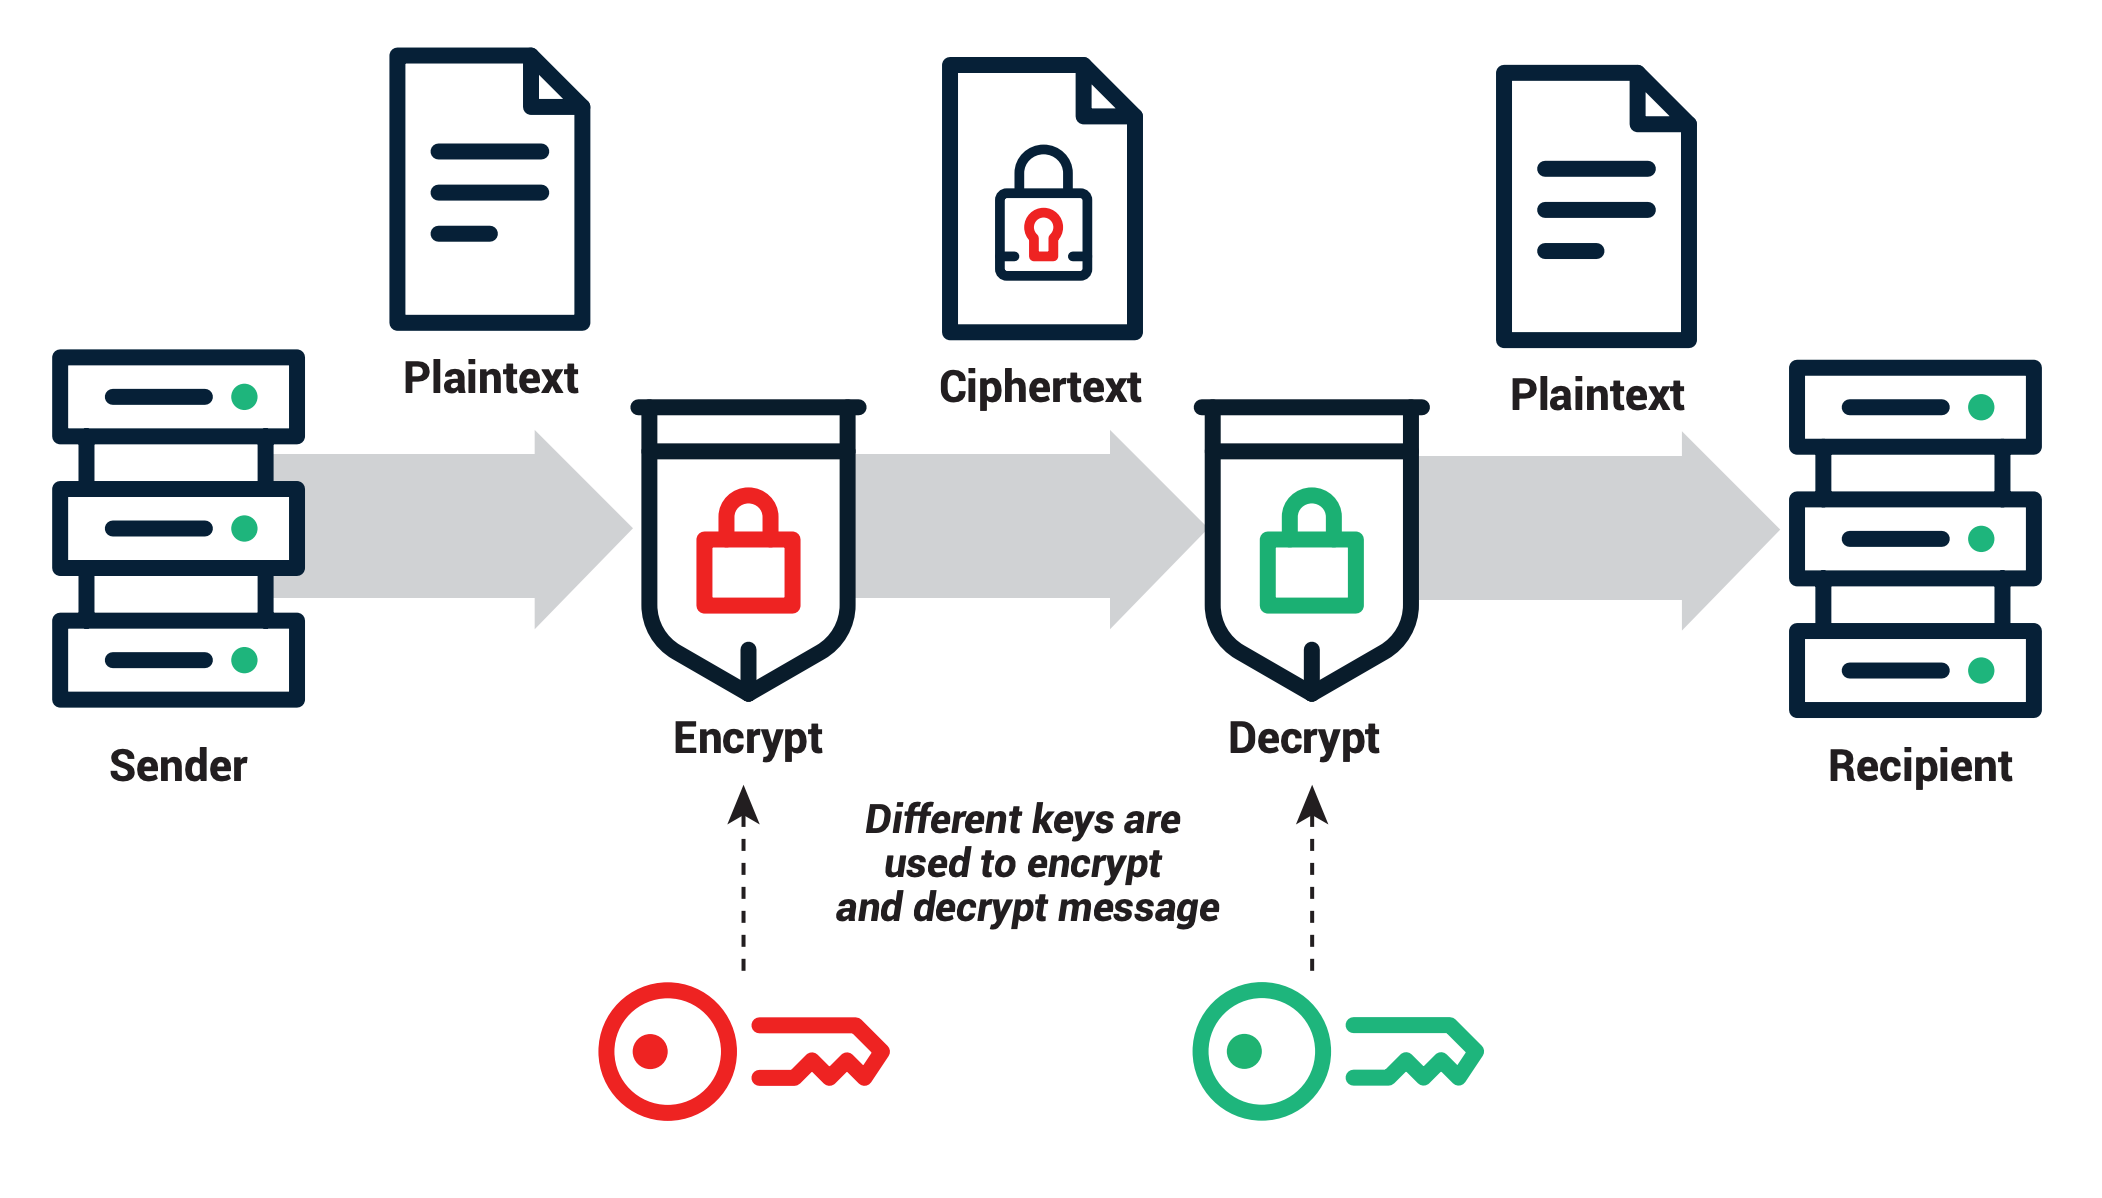
\includegraphics[width=\textwidth]{rsa.png}
    \end{center}
\end{frame}

\begin{frame}[fragile]{Setup your \texttt{git} account}
\begin{enumerate}
    \item Generate a \texttt{SSH} keypair: \texttt{ssh-keygen}
    \item Get your newly generated \texttt{SSH} public key:
    \begin{lstlisting}
cat ~/.ssh/id_rsa.pub # Print.
clip < ~/.ssh/id_rsa.pub # Copy to clipboard.
    \end{lstlisting}
    \item Go to \url{https://github.com/settings/keys} and add the new key to your user account.
    \item Configure your machine:
    \begin{lstlisting}
git config --global user.name "Name Surname"
git config --global user.email "name.surname@email.com"
    \end{lstlisting}
\end{enumerate}
\end{frame}

\begin{frame}[fragile]{Clone the course repository}
\begin{enumerate}
    \item Clone the APSC repository:
    \begin{lstlisting}
git clone --recursive \
    git@github.com:pacs-course/pacs-examples.git
    \end{lstlisting}
    \item Go to \texttt{pacs/Examples} and follow the instructions.
    \item Go to \texttt{pacs/Examples/src/Utilities} and run
\begin{lstlisting}
make
make install
\end{lstlisting}
\pause
    \item \textbf{Have fun!}
\end{enumerate}
\end{frame}

\section{Exercise}
\begin{frame}{Exercise}
Given a \texttt{C++} source file implementing the \texttt{main()} function, write a \texttt{Bash} script that:
\begin{itemize}
\item checks if the source file exists;
\item if it does, the script invokes the \texttt{g++} compiler to generate the corresponding executable;
\item if it does not, an error message is printed to standard error.
\end{itemize}
\end{frame}

\begin{frame}[fragile]{Exercise (solution)}
Content of \texttt{compile.sh}:
\begin{lstlisting}
    if [[ "$#" -ne 2 ]]; then
        echo "Illegal number of parameters." >&2
        exit 1
    fi
    
    filename_src=$1  # First command-line argument.
    filename_exec=$2 # Second command-line argument.
    
    if [[ -e ${filename_src} ]]; then
        g++ ${filename_src} -o ${filename_exec}
    else
        echo "Filename ${filename_src} does not exist!" >&2
        exit 1
    fi
\end{lstlisting}
\vfill
How to use it:
\begin{lstlisting}
    chmod +x compile.sh
    ./compile.sh source_file.cpp main
\end{lstlisting}
\end{frame}
\end{document}
